\scanpage{44}
A) Algebraic group \deleted{\unsure{$G$|$E$}}\unsure{[|(}reductive] $G$ over $\mathbb{Q}$

B) principal bundle with integrable connection $\unsure{P|\mathbb P}$ over $G_S$

% slanted; marginal brace extends alongside C) and D)
\margin{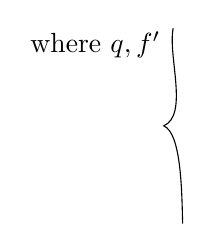
\begin{tikzpicture}[x=1cm,y=1cm,baseline=(current bounding box.north)]
\node[anchor=north east,inner sep=1pt] at (-.09,0) {where $q,f'$};
\draw (.03,0) .. controls (-.04,-.35) and (.23,-1.10) .. (-.09,-1.24)
.. controls (.13,-1.33) and (.14,-2.05) .. (.15,-2.48);
\end{tikzpicture}}
C) Restriction of the group $G_{\mathbb{C}}^{\mathrm{an}}$ to $G(\mathbb{Q})$ in $P_{\mathbb{C}}^{\mathrm{an}}$, whence
\diagram{\begin{tikzcd}[ampersand replacement=\&,column sep=2em]
\text{covering}\quad\deleted{\unsure{\bar S|\widetilde S}}\quad\widetilde P \arrow[r,hook,"p"] \& P_{\mathbb{C}}^{\mathrm{an}} \arrow[r] \& P
\end{tikzcd}}

D) Holomorphic map
\[
f:\widetilde P\longrightarrow\unsure{\gamma|\mathscr{Y}}_G
\]
satisfying $f(xg)=g^{-1}f(x)$ $(x\in\widetilde P,\,g\in G(\mathbb{Q})$ and compatible with the data B) and $p$ of C).

E) Restriction of $\widetilde P\mathbin{\times}^{G(\mathbb{Q})}G(\mathcal A)$ to $S$, with compatibility relative to $G/G^{\circ}$.

NB Knowledge of A) B) C) and of $f(\xi_0)$, where $\xi_0\in\widetilde P$ is above the generic point of $S$ [\uline{Condition} may \uline{be superfluous}] \margin{??}should in principle make it possible to reconstruct the whole of D) and E) [when one knows \deleted{that} that the data come from a category of motives $M$].

% slanted; boxed marginal note
\margin{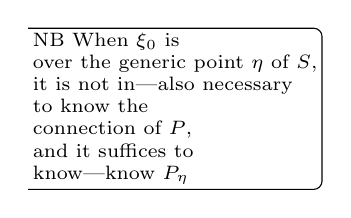
\begin{tikzpicture}[baseline=(current bounding box.north)]
\node[align=left,inner sep=1.5pt,font=\scriptsize] (note) {\uline{NB} When $\xi_0$ is\\
over the generic point $\eta$ of $S$,\\
it is not \deleted{\unsure{in|also}} necessary\\
to know the\\
connection of $P$,\\
and it suffices to\\
\unsure{know|know} $P_{\eta}$};
\draw[rounded corners=3pt] (note.north west) -- (note.north east) -- (note.south east) -- (note.south west);
\end{tikzpicture}}
\uuline{Analytic formula for continuation of $f$} ?

\uuline{Relations between D) and E)} ?? [\unsure{Jugendtraum|Jugend traum} ?]
% archive sheet number: 43
